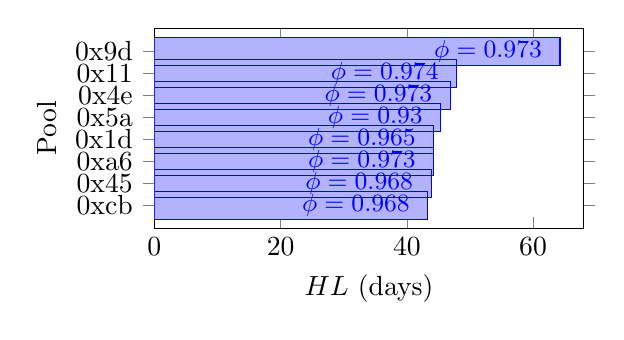
\begin{tikzpicture}
  \begin{axis}[
    xbar,
    width=0.58\textwidth,
    height=0.34\textwidth,
    xlabel={$HL$ (days)},
    ylabel={Pool},
    % order bars by HalfLife (largest at top), matching the new results:
    symbolic y coords={0x9d,0x11,0x4e,0x5a,0x1d,0xa6,0x45,0xcb},
    ytick=data,
    y dir=reverse,
    xmin=0,
    xmax=68,
    bar width=10pt,
    enlarge y limits=0.15,
    point meta=explicit,
    nodes near coords={$\phi=\pgfmathprintnumber[fixed,precision=3]{\pgfplotspointmeta}$},
    nodes near coords style={
        anchor=east,
        xshift=-3pt,
        font=\small
    },
  ]

    % (half-life, pool-id) [mean phi]
    \addplot coordinates {
      (64.26,0x9d) [0.973] % 9d  WBTC/USDT
      (47.89,0x11) [0.974] % 11  WETH/USDT 0.05%
      (46.88,0x4e) [0.973] % 4e  WETH/USDT 0.30%
      (45.39,0x5a) [0.930] % 5a  AAVE/WETH 0.30%
      (44.28,0x1d) [0.965] % 1d  UNI/WETH 0.30%
      (44.28,0xa6) [0.973] % a6  LINK/WETH 0.30%
      (43.84,0x45) [0.968] % 45  WBTC/WETH 0.05%
      (43.33,0xcb) [0.968] % cb  WBTC/WETH 0.30%
    };

  \end{axis}
\end{tikzpicture}
